
\begin{abstract}
Kolmogorov complexity measures the amount of information in data, but does not distinguish structure from noise. Kolmogorov's definition of the \emph{structure function} was the first attempt to measure only the structural information in data, by measuring the complexity of the smallest model that allows for optimal compression of the data. Since then, many variations of this idea have been proposed, for which we use \emph{sophistication} as an umbrella term. We describe two fundamental problems with existing proposals, showing many of them to be unsound. Consequently, we put forward the view that the problem is fundamental: it may be impossible to objectively quantify the sophistication.
\end{abstract}

\section{Introduction}\enlargethispage{3\baselineskip}

Kolmogorov complexity gives us a sound definition of the amount of information contained in a binary string. It does not, however, capture what most people would consider complexity. For example, a sequence of a million coin flips will almost certainly have maximal Kolmogorov complexity, even though there is nothing complex about flipping a coin repeatedly. Many scholars have defined additional measures in the spirit of Kolmogorov complexity, aimed at quantifying not \emph{all} information in a binary string, but only the \emph{meaningful}. While this concept has been given many names, we use \emph{sophistication} as an umbrella term. In this paper, we investigate two serious problems with sophistication. We conclude with two arguments suggesting the problems are fundamental, explaining our belief that sophistication cannot be defined in a satisfactory manner.

The Kolmogorov complexity $C(x)$ of a binary string $x$ is, informally, the length of the shortest computer program to print $x$. This length depends on the choice of programming language, but, by the invariance theorem \cite[Section~2.1]{li1993introduction}, only by a constant, independent of $x$. For sufficiently complex objects, the choice of programming language becomes irrelevant and Kolmogorov complexity becomes an \emph{objective} measure. A definition of sophistication $S(x)$ in the spirit of $C(x)$ should have similar guarantees:

\begin{enumerate}
\item $S(x)$ should count the bits required for an effective description of the structural properties of a binary string.
\item An analogue of invariance should hold: there must be strict limits on how much sophistication can be affected by a change in programming language.
\item There should be no constant $c$ such that $S(x)\le c$ for every input $x$. If sophistication is bounded, then knowing its value under one programming language provides no constraints on its value under another language (except it is also bounded). 
\item Similarly, there should be no constant $c$ such that $\left | C(x)-S(x)\right |\le c$ for all $x$, because then sophistication would be equivalent to Kolmogorov complexity. 
\end{enumerate}
There have been many proposals for such a measure, all based on a \emph{two-part code}: we encode a \emph{model} in the first part of the code, which is interpreted as a representation of $x$'s structural properties. The model does not fully specify $x$, but when combined with the second part of the code, which specifies the noise, the original string becomes fully determined.\footnotemark

\footnotetext{Some variants deviate from the two-part coding format, see Section~\ref{section:other}.}

For any string $x$, there may be many different two-part codes. The total length can never be less than the Kolmogorov complexity, but it can come close. Figure~\ref{fig:diagram} illustrates the principle. The key to sophistication is to take the representations that come close to the Kolmogorov complexity, the \emph{candidates}, and define the sophistication as the size of the smallest model in this set. However, for most definitions, we can prove that they fail one of the conditions above. For others, we cannot \emph{prove} they conflict with our requirements, but we show these methods only assign substantial sophistication to strings that require an enormous amount of processing to construct. 

\begin{figure*}[tb]
  \vspace{-2\baselineskip}
  \centering
  \begin{minipage}{0.40\textwidth}
     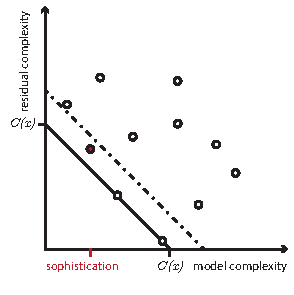
\includegraphics[width=\textwidth]{./img/sophistication.pdf}
  \end{minipage}
  \begin{minipage}{0.40\textwidth}
     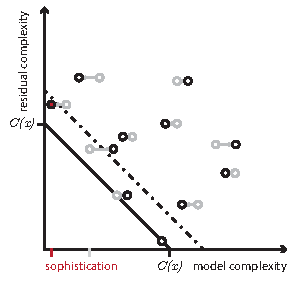
\includegraphics[width=\textwidth]{./img/sophistication-jump.pdf}
  \end{minipage}
  \caption{\small (left) Two-part representations of $x$ by the two components of their code. The Kolmogorov complexity $C(x)$, appearing as a black diagonal, provides a lower bound on the total codelength. We consider only representations that are close to this optimum---called \emph{candidates}---with the threshold represented by a dashed line. The size of the smallest model below the threshold is the sophistication of the data. (right) The same image, after a constant perturbation in the model complexity caused by a change in numbering.}
  \label{fig:diagram}
\end{figure*}\enlargethispage{3\baselineskip}

A valid definition of $S(x)$ must contend with two important issues. First, the details of the way the model is encoded are important. There are two technically distinct approaches; in one of these one has to deal with the so-called ``nickname problem'' that strangely remains unresolved in several publications. These definitions yield a sophistication that is highly dependent on the chosen programming language, unless special care is taken, as discussed in Section~\ref{section:indices}.

The second issue is that of striking the right balance between under- and overfitting, which we consider in Section~\ref{section:balance}. Overfitting is a common problem in statistics, that refers to the tendency to choose a complex model that provides a very good fit to the observed data, but does not generalise well to unseen data. In the case of sophistication, overfitting occurs if the model that determines the sophistication contains much or even all of the noise. In statistics, overfitting is often addressed by penalising complex models. In sophistication, however, such penalties tend to break the balance between structural information and noise, and lead to the opposite problem: underfitting.

Underfitting occurs when the selected model is simple, but fails to capture all structure in the data. This is also a problem for sophistication because the models under consideration are so powerful. In particular, in any programming language, there are programs that implement an interpreter for \emph{another} language. Such \emph{universal models} are \emph{simple}, since they can be described with a relatively small number of bits, yet are able to represent any data using a code within a constant from the Kolmogorov complexity. Such a two-part representation essentially encodes all information as noise. If complex models are penalized, then the problem becomes to make sure that universal models are not \emph{always} preferred for complex data. The usual workaround is to restrict the set of allowed models, for instance to total functions. While this excludes universal models, it is questionable whether it adequately solves the problem of underfitting in general.

Finally, in Section~\ref{section:conclusion} we argue that while two-part coding can yield useful insights into the structure of the data and identifies some models as poor representations, it is probably not possible to objectively separate structure from noise and identify a \emph{single} model as ``best'': many models of different complexities may be reasonable representations. Rather than doggedly trying to ``fix'' this property of algorithmic statistics, we propose embracing the idea that the data allows for multiple, equivalent interpretations of which information is structured, and which is random, and that there is no such thing as sophistication.

\section{Notation}\enlargethispage{3\baselineskip}
The following notation allows us to generalize across all definitions and variants, save the occasional exception which we will highlight individually.

Let $\B = \{0,1\}^*$. We deal with partial computable functions $f: \B \times \B \to \B$, which we
also call \emph{models}. $f$ is called \emph{prefix} if $\text{dom}_z(f)~=~\{y~:~f(y,~z)~\neq \infty\}$, is a prefix free set for all $z$, i.e. no string in $\text{dom}_z(f)$ is a prefix of another. A function $f$ is \emph{total} if $\forall_z \text{dom}_z(f) = \B$. In most cases, we do not use the second argument, and let $f(x) = f(x, \epsilon)$.

A \emph{numbering} is an enumeration of the partial computable functions, denoted by $\psi_1, \psi_2, \ldots$ or simply $\psi$. We fix one canonical numbering $\phi$, chosen to be \emph{effective}: ie. given $i$ and $y$, we can effectively compute $\phi_i(y)$. We call a numbering $\psi$ \emph{acceptable} if there exist total, computable functions $a, b: \N \to \N$ with $\forall: i$, $\phi_i = \psi_{b(i)}$ and  $\psi_i = \phi_{a(i)}$.

A \emph{model class} is a set of indices in a numbering $\psi$. We define four classes:
\begin{itemize} 
  \item The indices of the partial computable functions $\C=\N$.
  \item The total functions $\T=\{i:\tn{$\psi_i$ is total}\}$. Note that $\T$ is not computably enumerable.
  \item $\K$ is an enumerable set such that $\{\psi_i:i\in\K\}$ is the set of all partial computable prefix functions.
  \item The finite sets: $\F$ is an enumerable set such that $\{\psi_i:i\in\F\}$ is the set of uniform codes for all finite sets.\footnote{A uniform code for a set $F$ is a surjective prefix function $f:\{0,1\}^{\lceil\log|F|\rceil}\to F$.}
\end{itemize}

Let $\br{x}$ denote the prefix-encoded representation for $x$. We require that the mapping satisfies $|\br{x}| = |x|+O(\log|x|)$ (see eg. \cite[Section~1.4]{li1993introduction}). To simplify notation, we will sometimes conflate natural numbers and binary strings, implicitly using the ordering $(0, \epsilon)$, $(1, 0)$, $(2, 1)$, $(3, 00)$, $(4, 01)$, \ldots  

For technical reasons, we deviate slightly from the traditional notation of Kolmogorov complexity: let $\M$ be a model class and $\psi$ an acceptable numbering, then let $C^{\M,\psi}(x\mid z)=\min\{|\bar\imath y|:\psi_i(y, z)=x,i\in\M\}$, with $C^{\M,\psi}(x) = C^{\M,\psi}(x\mid \epsilon)$. We omit the numbering when the distinction is not relevant. $C^\C(x)$ corresponds to the plain Kolmogorov complexity $C(x)$ and $C^\K(x)$ corresponds to the prefix-free version $K(x)$. Note that the notation $C^{\{i\}, \psi}(x)$ represents the smallest two-part description of $x$ using model $\psi_i$.

We use the principle of a numbering for the purpose normally served by the universal Turing machine. We prefer to work with numberings as it highlights an important issue: while Kolmogorov complexity is invariant to the choice of numbering this property does not immediately carry over to sophistication: for some treatments, the result is highly dependent on the chosen numbering, as we will see in the next section. 
 
\section{Inefficient indices}
\label{section:indices}

The simplest approach to sophistication would be to `open up' the Kolmogorov complexity and to see which program achieves the smallest description length: the program that \emph{witnesses} the Kolmogorov complexity. This witness is a two-part coding; it consists of a model and an input.

\begin{definition}[Index sophistication]
Let $\psi$ be an acceptable numbering. Let $\M$ be the model class from which candidates are chosen, and let $\Nm$ be the model class that determines the minimum achievable complexity. Let $c$ be a fixed constant. The \emph{index sophistication} is:
\[
\s_{\tn{index}}^{\M,\Nm,\psi,c}(x) = \min\left\{ |i| : C^{\{i\}, \psi}(x) \leq C^{\Nm, \psi}(x)+c,\;i \in \M\right\} \p
\]
When $\M = \Nm$, we will use $\s_\tn{index}^{\M,\psi,c}$. If the set over which the minimum is taken is empty, the sophistication is undefined.\label{definition:index}
\end{definition}
Koppel and Atlan's treatment \cite{koppelSoph1988,koppel1991almost}, where the name \emph{sophistication} originates, follows this basic logic, although it contains idiosyncracies like the use of monotonic models, and an extension to infinite strings. As the subsequent history of sophistication has discarded these, we will not discuss them here.

In \cite{antunes2009sophistication,antunes2013sophistication} Koppel's principle is limited to finite strings, with $\T$ as a model class. The definition is similar to $S_\tn{index}^{\T, \C,\psi,c}$, except the total complexity of a witness $(i,y)$ is measured as $|i|+|y|$ without the cost of delimiting the two. This difference is not relevant to the current discussion. The restriction to $\T$ is a common approach, which avoids underfitting, as discussed in the next section. 

\begin{lemma}\label{lemma:perverse}
Let $\s_\tn{index}^\psi$ denote any index sophistication with respect to numbering $\psi$ (with any choice for $\M$, $\Nm$ and $c$). There are acceptable numberings $\psi$ and $\xi$ such that for all $x$: $|\s_\tn{index}^\psi(x) - \s_\tn{index}^\xi(x)|\geq \tfrac{1}{2}\min\{\s_\tn{index}^\psi(x),\s_\tn{index}^\xi(x)\}$.
\end{lemma}
\begin{proof}
Let $z_i \in \B$ consist of $2^{i}-1$ zeroes followed by a one. Define $\psi, \xi$ such that $\psi_j(x) = \phi_i(x)$ for $j = z_{2i}$ and $\xi_j(x) = \phi_i(x)$ for $j = z_{2i+1}$, with all other functions returning $\infty$ for all inputs. Choose any $x$ and assume w.l.o.g. that $\s_\text{index}^\psi(x)\le \s_\text{index}^\xi(x)$. By construction, we have $2\s_\text{index}^\psi(x)  \leq \s_\text{index}^\xi(x)$.
\end{proof}\enlargethispage{3\baselineskip}
Thus, the length of the index is a very poor indicator of model complexity. For a robust measure, we define the complexity of a function $f$ as in \cite{grunwald2004shannon,vitanyi2004meaningful} by 
\begin{align}
C^{\M,\psi}(f) = \min\{C^{\M,\psi}(i):\psi_i=f\} \p \label{equation:function-complexity}
\end{align}
Lemma~\ref{lemma:invariance} in the appendix shows that $C^\C(f)$ and $C^\K(f)$ are invariant. Note that the perversely inefficient numberings of Lemma~\ref{lemma:perverse} are no issue for Kolmogorov complexity: we can use a UTM with a more efficient numbering as a model at only a constant penalty. For sophistication, however, the numbering is crucial.

There are two ways to use $C^\M(f)$ for more robust attempts to define sophistication. Confusingly, both are used in the literature. First, we can measure the complexity of the \emph{model} $\phi_i$ as $C^\K(\phi_i)$, which is then the size of the first part of a two-part code describing the data. This approach is used in  \cite{cover1985kolmogorov,gacs2001algorithmic,vitanyi2004meaningful,gellmann1996information}.

Second, we can stick to using the length of the index as the measure of sophistication, but restrict the allowed numberings to those that can represent a given function \emph{efficiently}. This approach is taken by Adriaans in \cite{adriaans2012facticity}, who defines \emph{facticity} as $\s_\text{index}^{\C,\psi,0}$, but only allows \emph{faithful} numberings. Formally, a faithful numbering has the property that $\forall i \exists j : \psi_i=\psi_j, |j|\le C^{\C}(\psi_j)+c$, for some constant $c$. Essentially, this means that a faithful numbering can represent a function $f$ with an index the same length as the Kolmogorov complexity $C^\C(f)$.

We prove in the appendix that---contrary to Adriaans' suggestion---there do exist faithful, acceptable numberings (Lemma~\ref{lemma:faithful-numberings}). However, even choosing a faithful numbering is not enough. The Kolmogorov complexity uses representations of the form $\bar\imath y$, with $\psi_i(y) = x$,  where the bar denotes some straightforward prefix encoding to delimit the model description $i$ from its input $y$. If we define a second prefix encoding $\tilde{\imath}$, with $|\bar\imath|-|\tilde\imath|$ unbounded, we can define a second representation $\bar u \tilde \imath y$, with $\psi_u(\tilde{\imath} y) = \psi_i(y)$, at a constant overhead $|\br{u}|$, and gain more than $|\br{u}|$ for sufficiently complex strings, resulting again in a bounded sophistication.

We continue with a sophistication that avoids the issues of inefficient indices and of inefficient prefix encodings. We change the definition of index sophistication so that its two-part representations use $C^\K(\phi_i)$ bits for the representation of the model. We first introduce the following notation for the $\M$-Kolmogorov complexity using such compact two-part representations:
\[
\Cc^{\M, \psi}(x) = \min\{ C^{\K, \psi}(\psi_i) + |y| :  \psi_i(y) = x, i \in \M\}\p
\]
For model classes $\K$ and $\C$ this is equivalent to the existing definition and invariant to the numbering. Note that again, we use $\Cc^{\{i\}, \psi}(x)$ to represent the smallest two-part code using model $\psi_i$.

\begin{definition}[Sophistication]
\[
S^{\M,\Nm,\psi,c}(x)=\min\left\{C^\K(\phi_i): \Cc^{\{i\}, \psi} \le \Cc^{\Nm,\psi}(x)+c, i\in\M\right\}.
\]
\end{definition}

\section{Balancing under- and overfitting}
\label{section:balance}

In the last section, we began to see the delicate balance between the two code components. We will study this balance, starting with the variant $S^{\K,\psi,c}$, which is not used in the literature, but helps to illustrate the issues we wish to discuss.

$\K$ has optimal representations with all but a constant part of the information in the input and it has optimal representations with all information in the model. The downside to this balance is that it becomes easy to show a lack of invariance. We can tweak the numbering so that models in a specific subset $\M'\subset\K$ become cheaper to represent by an arbitrary amount relative to others: we can ensure that a model in $\M'$ always determines the sophistication. For instance, if we let $\M'$ contain only a universal model we get a bounded sophistication.

\begin{theorem}[Underfitting]
Let $\M, \Nm$ be model classes with $\M \subseteq \Nm$ and let $\M$ contain a universal model $\phi_u$, with the property that $\exists c \forall i \in \Nm, x \in \B : \Cc^{\{u\},\phi}(x) \leq \Cc^{\Nm, \phi}(x)+ c$. Then, for some numbering $\psi$, $S^{\M,\Nm, \psi,c}$ is bounded. \label{theorem:underfitting}
\end{theorem}
This problem is well known and many treatments avoid it by restricting the model class. Less well known, perhaps, is that the same holds in the other direction:  if $\M'$ is the set of \emph{singleton} models---those models that output a single $x$ for an empty input---we get a sophistication equal to the Kolmogorov complexity.

\begin{theorem}[Overfitting]
Let $\X \subseteq \B$. Let $\M \subseteq \Nm \subseteq \K$ be model classes where for every $x\in\X$ there is a singleton model $i\in\M$ with $\phi_i(\epsilon)=x$. Then there is a numbering $\psi$, and a constant $c$, such that for all $x\in\X$ we have $C^\K(x)-S^{\M,\Nm,\psi,c}(x) \leq c$.\label{theorem:overfitting}
\end{theorem}
The proofs of both theorems rely on a simple principle: there exist numberings which have the effect of penalizing $C^\K(\phi_i)$ for any model outside $\M'$ by an arbitrary constant amount. We can use this to effectively `push' these models outside of the range of candidates, ensuring that, under this numbering, a model in $\M'$ always determines the sophistication. The requirements for $\M'$ are somewhat complex. The following lemma gives a set of sufficient conditions.

\begin{lemma}
\label{lemma:thecoolone}
Let $\M$ and $\Nm$ be any model class, let $\X$ be any set of binary strings and let $D:\B\to\N$ be a partial computable decoding function with a prefix-free domain that maps function descriptions to their indices in $\phi$. Let $\M'= \tn{range}(D)$. Further assume there is a constant $c$ such that:\\
\-\hspace{1cm}(a) $\forall_{m\in\M'}:\min\{|p|:\phi_{D(p)}=\phi_m\}\le C^{\K,\phi}(\phi_m)+c$\\
\-\hspace{1cm}(b) $\forall_{x\in\X}: \Cc^{\M', \phi}(x) - \Cc^{\Nm, \phi}(x) \le c$.\\
Then, there is a $\psi$ such that if $S^{\M,\Nm,\psi,k}(x)$ is defined, then $S^{\M,\Nm,\psi,k}(x) = S^{\M',\Nm,\psi,k}(x)$ up to a constant. 
\end{lemma}
\begin{proof}\enlargethispage{2\baselineskip}
Pick any $x \in \X$. Let $f$ and $g$ be $\phi$-indices such that $f \in \M'$ and $g \notin \M'$ nor is $\phi_g$ equivalent to any function indexed by $\M'$. Furthermore let $\Cc^{\{f\}, \phi}(x)$ and $\Cc^{\{g\}, \phi}(x)$ both be within a constant $q$ of $\Cc^{\Nm,\phi}(x)$. Assumption (b) ensures that $\M'$ always provides such an $f$. 

We will show that for every integer $r$, there is a numbering $\psi$ such that $\Cc^{\{g'\}, \psi}(x) - \Cc^{\{f'\}, \psi}(x) \geq r$ for all $x \in \X$, where $f'$ and $g'$ are the $\psi$-indices equivalent to $f$ and $g$. Thus, for large enough $r$, $\phi_g$ is eliminated as a candidate model, while $\phi_f$ remains in place. Thus, under $\psi$, a member of $\M'$ determines the sophistication, or the sophistication is undefined.

Let $d$ be a positive constant. We will show later how to choose it to achieve the required result. We define $\psi$ as follows:
\[
\psi_0(p) = 0^d 1 D(p), \;\;\;
\psi_{0^d1i}(p) = \phi_i(p), \;\;\;
\psi_j(\cdot) = \infty \;\text{if $j\neq 0$ and $j \neq 0^d1\ldots$}
\]
The key to the proof is the way that the function complexity $C^\K(\cdot)$ changes when we change the numbering from $\phi$ to $\psi$. For $f$, the value increases by no more than a fixed constant, but for $g$, it increases by a constant that we can arbitrarily increase by increasing $d$.

We will first show that for $f$, the value does not increase by more than a constant $c_f$. Assume w.l.o.g. that $0 \in \K$.
\begin{align*}
C^{\K, \psi}(\phi_f) &= \min\left\{|\bar \jmath q| : \psi_{\psi_j(q)} = \phi_f, j \in \K \right\} & \text{rewriting (\ref{equation:function-complexity})} \\
&\leq \min \left\{ |\overline{0} q| : \psi_{\psi_0(q)} = \phi_f \right\}& \text{choose $j=0$} \\
&= \min \left\{ |q| : \phi_{D(q)} = \phi_f \right\} + |\overline{0}| \\
&\leq C^{\K, \phi}(\phi_f) + c_f & \text{by assumption (a).}
\end{align*}
In order to show that for $g$, we can increase the difference by an arbitrary constant, we first show that, for any $z$ not in the range of $\psi_0$, the Kolmogorov complexity itself increases by at least $d$ when we switch from $\phi$ to $\psi$:
\begin{align}
C^{\K, \psi}(z) &= \min\left\{|\bi y| : \psi_i(y) = z, i \in \K \right\} & \text{by definition}\nonumber\\
&= \min\left\{|\overline{0^d1j} y| : \psi_{0^d1j}(y) = z \right\} & \text{since $z\notin \text{range}(\psi_0)$} \nonumber\\
&\geq \min\left\{|\bar \jmath y| : \phi_{j}(y) = z \right\} + d &\nonumber\\
&= C^{\K, \phi}(z) + d\p & \label{line:kolmogorov-switch}
\end{align}
We now show the increase in model complexity for $g$. First, assume $\phi_g \neq \psi_0$:
\begin{align*}
C^{\K,\psi}(\phi_g) &= \min \left\{C^{\K, \psi}(i) : \psi_i = \phi_g \right\} \\
&= \min \left\{C^{\K, \psi}(0^d1j) : \phi_j = \phi_g \right\} \\
&= C^{\K, \psi}(0^d1j) \\
&\geq C^{\K,\phi}(0^d1j) + d & \text{by (\ref{line:kolmogorov-switch})} \\
&\geq C^{\K,\phi}(j) - c_g + d &\text{since $C^\K(j) \leq C^\K(0^d1j) + c_0$}\\
&\geq C^{\K, \phi}(\phi_g) - c_g + d \p
\end{align*}
Now assume $\phi_g = \psi_0$. We have $C^{\K,\psi}(\phi_g) = \min\left\{C^{\K, \psi}(i) : \psi_i = \psi_0 \right\} \geq d$. This follows from the fact that the minimum is achieved either at $i = 0$ or at $i = 0^d1m$ with $m \notin \M'$. Neither have a representation using a function with a $\psi$-index without the $0^d1$ prefix.

Choosing $d \geq r + \max \left\{C^{\K,\phi}(\psi_0), c_g \right\} + c_f + 2q$ ensures that for both cases, we have $C^{\K, \psi}(\phi_g) \geq C^{\K, \phi}(\phi_g) + r + c_f + 2q$. While $C^\K(\psi_0)$ depends on the choice of $d$, we have $C^\K(\psi_0) \leq C^\K(d) + C^\K(D)$, up to a constant, which is in $O(\log d)$, so we can choose $d$ to satisfy the inequality.  

Finally, we can show the result: \belowdisplayskip=-26pt
\begin{align*}
&\Cc^{\{g'\}, \psi}(x) - \Cc^{\{f'\}, \psi}(x)\\
&=C^{\K, \psi}(\phi_g) + \min\{|y| : \phi_g(y) = x\} - C^{\K, \psi}(\phi_f) - \min\{|y| : \phi_f(y) = x\}\\
&\geq C^{\K, \phi}(\phi_g) + r + c_f + 2q + \min\{|y| : \phi_g(y) = x\} \\
&\quad\quad- C^{\K, \phi}(\phi_f) - c_f - \min\{|y| : \phi_f(y) = x\} \\
&= \Cc^{\{g\}, \phi}(x) - \Cc^{\{f\}, \phi}(x) + r + 2q\geq r \p\\
\end{align*}
\end{proof}
Theorems~\ref{theorem:underfitting} and \ref{theorem:overfitting} follow as corollaries. For Theorem~\ref{theorem:underfitting}:
\begin{proof}
Let $D$ be a prefix function as in Lemma~\ref{lemma:thecoolone} that returns the index of $u$ for the argument $\epsilon$ and $\infty$ for any other argument. That is, $\M' = \{u\}$. This construction satisfies the conditions 1 and 2 from Lemma~\ref{lemma:thecoolone}. Invoking it, we find that there exists an acceptable numbering $\psi$ for which $S^{\M,\Nm,\psi,k}(x) = S^{\M',\Nm,\phi,k}(x) + c$. Since $\M'$ contains only a single model, $S^{\M',\Nm,\phi, c}(x)$ is constant.
\end{proof}
And for Theorem~\ref{theorem:overfitting}:

\begin{proof}
Let $x$ be any string. Given a description of $x$, we construct some index $i$ such that $\phi_i(\epsilon) = x$ (a singleton for $x$). Thus, $C^{\K, \psi}(\phi_i) \leq C^{\K,\psi}(x)$ up to a constant. Likewise, given $\phi$ we can produce $x$, so that $|C^{\K,\phi}(\phi_i)-C^{\K, \phi}(x)|\le c$ for some constant $c$. 

We now define a computable function $D$ by $D(\bar\imath y)=j$ where $\phi_j(\epsilon) = \phi_i(y)$ and $i \in \K$, and let $\M'$ be its range.  We will show that the two conditions of Lemma~\ref{lemma:thecoolone} hold for the prefix function $D$.

(a) Let $f \in \M'$ with $\phi_f(\epsilon) = x$. Then $\min\{|p|:\psi_{D(p)}=\phi_f\}=\min\{|\bar\imath q|:\phi_i(q)=x\}=C^{\K}(x) \le C^{\K}(\phi_f)+c$. (b) On the one hand $\Cc^{\M',\psi}(x)\le C^\K(\phi_f)+|\epsilon|\le C^\K(x)+c$. On the other hand, the witness to $\Cc^{\M,\psi}(x)$ is an effective description of $x$, so $C^{\K}(x)$ is at most a constant larger. 

Now, by Lemma~\ref{lemma:thecoolone} there is a numbering $\psi$ such that we have $S^{\M,\Nm,\psi,k}(x) =S^{\M',\Nm,\psi,k}(x) + c$. We observed that $|C^{\K}(\phi_i)-C^{\K}(x)|\le c_0$ for all singletons, so $S^{\M',\Nm,\psi, k}(x)\ge C^{\K,\psi}(x)-c_0$. This proves the theorem.
\end{proof}

\noindent Thus, in this balanced sophistication, there is no invariance: all information can be seen as structure, or as noise, depending on the numbering. To avoid these issues, existing proposals upset the balance to exclude or penalize the universal models, and possibly the singleton models. 

\subsection{Overfitting}

We will now review the treatments in the literature that show overfitting. The first is the structure function, proposed by Kolmogorov, most likely the first attempt at separating structure from noise in an objective manner. Kolmogorov defined the following function, using the finite sets $\F$ as models:
\[
h_x(\alpha) = \min \left \{\log |F| : x \in F, C^\K(F) \leq \alpha \right \} 
\]
and suggested that the smallest set for which $C^\K(F) + \log|F| \leq C^\K(x) + c$ holds for some pre-chosen constant $c$, can be seen as capturing all the structure in $x$ \cite{cover1985kolmogorov}. This is equivalent to the sophistication $S^{\F,\K,\psi,c}(x)$. Theorem~\ref{theorem:overfitting} shows there are numberings for which this sophistication is always equal to $C^\K(x)$. Thus, either this is true for all numberings, or this sophistication is not invariant.
 
In \cite{gacs2001algorithmic} the structure function is extended to an \emph{algorithmic sufficient statistic}. This is, again, essentially the witness to the sophistication $S^{\F,\K,\psi,c}(x)$. A probabilistic version is also introduced, which uses the model class $\mathcal P$, which indexes the set of functions that compute computable probability semimeasures up to a multiplicative constant error, yielding $S^{{\mathcal P}, \K, \psi, c}(x)$. For both, Lemma~\ref{theorem:overfitting} gives us a numbering such that the singleton is always the minimal sufficient statistic.

It may be argued that the slack parameter $c$ in the sophistication, which determines the allowed gap between a candidate representation and the complexity, should depend on the numbering, but this dependence has not been mentioned in the literature and there is no obvious method to choose this constant for a given numbering. 

In traditional statistics, overfitting is often addressed by a penalty on complex models. As we have seen, a strong penalty, such as the one imposed by an inefficient prefix encoding of the model, will cause underfitting. A more subtle approach is to allow descriptions that are not self-delimiting. The gap between the smallest self-delimiting description and the smallest non self-delimiting description grows without bound 
\cite[Section~4.5.5]{li1993introduction}, so that some information ends up in the noise, since placing all information in the model results in a self-delimiting, and thus non-optimal description. This eliminates the singletons as viable candidates. This approach is taken by Vit\'anyi \cite{vitanyi2004meaningful} and by Adriaans \cite{adriaans2012facticity}. Such measures reduce the overfitting problem, but they only increase the tendency to underfit. We also pay the price that the models can no longer be equated with probability measures, weakening the link to traditional statistics.

\subsection{Underfitting}
\label{section:underfitting}

Universal models are a widely acknowledged problem for sophistication, and most proposals avoid them by limiting the allowed models to exclude them. It is known that there are strings $x$ for which $S^{\F, \K, \psi, c}(x)$, $S^{\T, \psi, c}(x)$ and $S^{\T, \K, \psi, c}(x)$ are close to $|x|$ (up to a logarithmic term). Proofs can be found in \cite{gacs2001algorithmic}, \cite{antunes2009sophistication} and \cite{vitanyi2004meaningful} respectively. These are the \emph{absolutely non-stochastic strings} \cite{shen1983concept}. The existence of these strings is independent of the numbering. 

However, the problem of the singletons remains. Only one model class eliminates both the singletons and the universal model: $\T$. The only proposal we are aware of that uses an efficient model representation \emph{and} excludes the universal models \emph{and} excludes the singletons is: $S^{\T,\K,\psi,c}$, from \cite{vitanyi2004meaningful}. While this avoids our proofs of boundedness, there is no evidence that $S^{\T,\K,\psi, c}$ is actually invariant.

While high sophistication strings exist for $S^{\T,\K,\psi, c}$, they may not conform to sophistication's motivating intuition. To show this, we use the concept of depth:

\begin{definition}[Depth\cite{bennett1988logical,antunes2006computational}]\belowdisplayskip=-12pt
Let $U$ be some universal Turing machine, so that $U(\bar\imath y) = \phi_i(y)$. Let $U^t$ be a simulation of this machine, which is allowed to run for at most $t$ steps, and returns $0$ if it has not yet finished at that point. Let $C^\M_t(x) = \min\{|\bar\imath y| : U^t(\bar\imath y) = x, \phi_i \in \M\}$. The \emph{$c$-depth} is $d^{\M,c}(x) = \min \left\{t : C^\M_t(x) - C^\M(x) \leq c \right\}$.
\end{definition}
Deep strings are those that can only be optimally compressed with a great investment of time. We note that it is exceedingly unlikely that a deep string is sampled from a shallow distribution \cite{bloem2014safe,bennett1988logical}. 
 
\begin{theorem}
Let $A(n)$ be the single-argument Ackermann function and $c_d$ some constant. For all $k$, there is a numbering $\psi$ such that for all strings with depth $d^{\C,c_d}(x) \leq A(C^\C(x))$ the sophistication $S^{\T, \K, \psi, k}(x)$ is bounded.\label{thm:depth}
\end{theorem}

\begin{proof}
Let $U(\bar\imath y)$ be some universal Turing machine, and let $U^A(\bar\imath y)$ be a simulation of that machine which outputs $0$ if the number of steps taken exceeds $A(|\bar\imath y|)$. Let $u$ be the index of the function $U^A$ in the standard enumeration.

Let $D(\epsilon) = u$. We can instantiate Lemma~\ref{lemma:thecoolone} with $D$, $\M' = \{u\}$ and $\X = \{x : d^{\C,c_d}(x) \leq A(C^\C(x))\}$. This tells us that there exists a numbering $\psi$ for which $S^{\T, \K,\psi,k}(x) = S^{\M', \K, \psi, k}(x) + |\bar0| \leq c$ for all $x \in \X$.
\end{proof}

\noindent This shows that while high-sophistication strings exist, they do not behave as expected. Consider a string that is typical for a shallow model, say some elaborate probabilistic automaton. Under $S^{\T,\K, \psi,c}$, no matter how high the complexity of the automaton, the sophistication is bounded. We could encode the collected works of Shakespeare in its transition graph, and this information would be counted as noise. Any structure simple enough to be exploited within the time bound of the Ackermann function will not be seen as `meaningful information'. Only structure so deep that it would take beyond the lifetime of the universe to decompress would count towards sophistication. In the remainder we will refer to strings $x$ with $d^{\C,c}(x) \leq A(C^\C(x))$ as \emph{shallow} strings. Note that any string whose shortest program can be run in any time bound represented by a primitive recursive function is shallow. 

The relation between $S(x)$ and $d(x)$ is also investigated in \cite{antunes2013sophistication}, where it is shown that within a logarithmic error term on the sophistication and the slack, they are identical. Our point is not the similarity between the two, but that for all practical strings, the sophistication is bounded. This contradicts the intuition that sophistication measures structure, as it seems to suggest that all strings we can possibly hope to understand or generate contain no structure, save a constant amount. The alternative is that under other numberings these strings \emph{do} have structure, but then the sophistication is not invariant.

As for the strings with high sophistication, they have the property that they can be compressed far better with partial functions than with total: they are non-typical for the model class $\T$. This suggests that the `non-stochastic' property of strings with high sophistication \cite{shen1983concept,vereshchagin2004kolmogorov} says more about depth and totality than it does about structure and noise.

\subsection{Other variants} 
\label{section:other}

By moving away from the idea of two-part coding, the mechanics of lemma~\ref{lemma:thecoolone} can be avoided. In \cite{mota2013sophistication}, the \emph{naive sophistication} is introduced. We will define a generic version, parametrized by model class. Let $C_{\psi_i}(x) = \min\left\{|y| : \psi_i(y) = x\right\}$. Then we define the \emph{naive sophistication} as:
\[
\s_\tn{naive}^{\M, \psi, c}(x) = \min\left\{C^{\K, \psi}(\psi_i) : C_{\psi_i}(x) - C^{\K,\psi}(x\mid i) \leq c, i \in \M \right\} \p
\]
\noindent The condition now is not that the two-part code length is minimal, but that the \emph{randomness deficiency} $C_{\psi_i}(x) - C^{\K,\psi}(x\mid i)$ is less than a constant. $S_\tn{naive}^{\F,\psi,c}(x)$ corresponds to the version in \cite{mota2013sophistication}. The switch to the randomness deficiency avoids Theorem~\ref{theorem:overfitting}, but we end up with the same problem as in Theorem~\ref{thm:depth}: for shallow strings $S_\tn{naive}^{\T, \psi, c}$ is defined by the model $U^A$, and thus bounded.

We cannot show that $S_\tn{naive}^{\F, \psi, c}(x)$ is bounded for shallow strings, but this is only a consequence of the use of sets, not of the switch to randomness deficiency as a condition. \emph{Any} set sophistication is necessarily lower-bounded by the function $\tn{set}(x) = \min\left\{C^\K(F) : x \in F\right\}$ and if this function were bounded, it would suggest that a finite amount of finite sets contained all strings.
\begin{theorem}
Let $\psi$ be \emph{any} acceptable numbering. Then for all shallow $x$ and large enough $c$, $S_\tn{naive}^{\T,\K,\psi,c}(x)$ is bounded and for come constant $c_F$, we have:\belowdisplayskip=-12pt
\[
\tn{set}(x) \leq S_\tn{naive}^{\F,\K,\psi,c}(x) \leq C^{\K,\psi}(C^{\K, \psi}(x)) + c_F \p
\]\label{theorem:naive}
\end{theorem}
\begin{proof}
Let $\psi$ be any acceptable numbering. Let the Turing machine $U$ be defined as $U(\bi y) = \psi_i(y)$ if $i \in \K$, and $U(\bi y) = \infty$ otherwise. Let $U^A$ be derived from $U$ as in section in Section~\ref{section:underfitting} and let $\phi_u$ compute $U^A$.

For the first part we have $C_{\psi_u}(x) - C^{\K, \psi}(x\mid u) \leq c_0$ for some $c_0$, thus for large enough $c$, $\s_\text{naive}^{\T,\psi,c}(x) \leq C^K(\psi_u)$. For the second part, let $C^{\K,\psi}(x) = k$ and $F^A_k = \{x \mid \exists p : U^A(p) = x, |p| = k\}$. $|F^A_k| \leq |\{p : |p| = k\}|$, so that $\log |F^A_k| \leq k$, which gives us $\log |F^A_k| - C^{K, \psi}(x \mid F^A_k) \leq c_1$. Thus, for large enough $c$, $\s_\text{naive}^{\F,\psi,c}(x) \leq C^K(F^A_k)$. From a description of $k$, we can compute $F^A_k$ with a finite program, so that $C^{\K,\psi}(F^A_k) \leq C^{\K,\psi}(k) + c_F$, which completes the proof.
\end{proof}
Note that the constant $c$ only needs to be large enough to ensure that $C^{\K,\psi}(x) - C^{\K,\psi}(x\mid u) \leq c$ and $C^{\K,\psi}(x) - C^{\K,\psi}(x\mid F^A_k)\leq c$. Since $u$ and $F^A_k$ are generally of no value in computing $x$, $c$ is likely very small.

Another approach is the \emph{coarse sophistication} \cite{antunes2009sophistication}, defined in \cite{mota2013sophistication} as:
\[
S^{\M,\Nm,\psi}_\tn{coarse}(x) = \min_c\left\{S^{\M,\Nm,\psi,c}(x) + c \right\} \p
\]
Again, this variant avoids the pitfalls of Theorem~\ref{theorem:overfitting}. If there are candidates that are as good as the singletons but with smaller size by more than a constant, the constant penalty $c$ will eventually be much less than the gain for the simpler witness, and the singletons will not determine the coarse sophistication. The coarse sophistication is within a logarithmic term of the busy beaver depth \cite{antunes2009sophistication}. As with the naive sophistication, we can show that for shallow strings, the total function version is bounded, and the set version grows very slowly:
\begin{theorem}
Let $\psi$ be \emph{any} acceptable numbering. For all shallow $x$, $\s_\tn{coarse}^{\T,\K,\psi}(x)$ is bounded and there is a constant $c_F$ such that:\belowdisplayskip=-12pt
\[
\text{set}(x) \leq s_\tn{coarse}^{\F,\K,\psi}(x) \leq 2 C^{\K,\psi}(C^{\K,\psi}(x)) + c_F \p
\]\label{theorem:coarse}
\end{theorem}
\begin{proof}
Let $\psi$ be any acceptable numbering and define $U^A$, $\phi_u$ and $F^A_k$ as in the proof of Theorem~\ref{theorem:naive}. For the first part, we know that for some constant $c_0$, $\Cc^{\{u\}, \psi}(x) \leq \Cc^{\K,\psi}(x) + c_0$ so that $S^{\T, \K,\psi,c_0}(x) \leq C^{\K,\psi}(\phi_u)$, thus $S_\text{coarse}^{\T,\K,\psi}(x) \leq C^{\K,\psi}(\phi_u) + c_0$. For the second part, we know that for some $c_1$, $C^{\K,\psi}(F^A_k) + \log|F^A_k| \leq C^{\K,\psi}(k) + C^{\K,\psi}(x)+ c_1$, so that $S^{\F,\K,\psi,C^\K(k)+c_1}(x) \leq C^{\K,\psi}(F^A_k)$. Thus, $S_\tn{coarse}^{\F,\K,\psi}(x) \leq C^{\K,\psi}(F^A_k) + C^{\K,\psi}(k) + c_1 = 2 C^{\K,\psi}(C^{\K,\psi}(x)) + c_F$.
\end{proof}
In \cite{vereshchagin2013algorithmic}, Vereshchagin proposes a \emph{strongly algorithmic sufficient statistic}. Where the regular algorithmic sufficient statistic $F$ from \cite{gacs2001algorithmic} has $C^\K(F\mid x)$ constant, the strong variant imposes the stronger requirement that $C^\T(F\mid x)$ is also constant. This reduces the problems of underfitting discussed in this section, but since $C^\T(\{x\}\mid x)$ is bounded, by Theorem~\ref{theorem:overfitting}, overfitting remains a problem: there exist numberings under which the singletons are the only candidates.

Finally, \emph{effective complexity} \cite{gellmann1996information}, proposed by Gell-Man and Lloyd, was formulated from the perspective of physics, but fits the mold of sophistication. The model class consists of all computable probability distributions on finite sets. The complexity of the model is measured by its Kolmogorov complexity, avoiding the problems of Section~\ref{section:indices}. Theorem~\ref{theorem:overfitting}, however, still applies to effective complexity. Unlike other sophistication measures, it is not the candidate with the smallest model which is chosen, but the one which reproduces the data within the shortest time. Thus, if there are multiple candidates, this approach would likely favor the singletons. In \cite{gell2004nonextensive}, the authors abandon this approach, and note that the choice from the set of candidates is a subjective one, which depends on context, which is in line with the view we express in the next section.

\section{Discussion and conclusion}
\label{section:conclusion} 

We have criticized existing measures of sophistication and shown technical problems with all of them. But that does not in itself mean that it should be impossible to come up with a sound measure. The common intuition, starting with the structure function, appears to be that the crucial property is whether a string is typical for a model, and that this typicality can be tested: another random choice from that model should select a string with the same structure. This idea is bold, but not  unreasonable. Nevertheless, we offer the opinion that such a clean-cut separation \emph{cannot} be made to work. We provide two arguments.

For the first argument, we take a generative perspective. We can generate data from a model $\phi_i, i \in \K$, by feeding it random bits until it produces an output. We will call the resulting probability distribution $p_i$. Call a sophistication \emph{consistent} if, for sufficiently large data, it reflects the complexity of the source of the data. Now, let $\phi_u(\bar\imath y)=\phi_i(y)$ and sample from $p_u$. Then the initial bits will determine the prefix encoded index $\bar\imath$ of the function $\phi_i$ that $\phi_u$ will subsequently emulate, and the remaining bits are used as inputs to $\phi_i$. We now ask, what should be the sophistication of the resulting data? 
 
Certainly, if we have to judge based only on the data, we cannot exclude the possibility that the data was sampled from $p_u$: after all, it was. Yet, neither can we deny that it may have came from $p_i$, as again, it did!  Eliminating the universal models does not solve this problem: the same argument holds if $\phi_u$ indexes, for instance, only those models computable by finite automata. \emph{Any} model that dominates a set of other models creates this kind of ambiguity.

Consider the following metaphor. We are given a a bitmap image of the painting \emph{Impression of a Sunrise}. There are many good models for this string, from very generic to very specific. Sophistication suggests that we can choose one of these as the objective, intrinsic model of the data. The universal model says that it is `some compressible, finite object'. Another might say that it is `an image'. Even more specific would be `a painting', `a Monet', or specifically `the painting \emph{Impression of a Sunrise}'. A sound sophistication should be able to select one of these as the proper representation of structure in the data, and disqualify the others as over- or underfitting. But how should we be able to say that the data is intrinsically more of a painting than an image? More of a Monet than a painting? Intuitively, such distinctions require further assumptions, or a second sample from the same distribution.

The second reason we doubt sophistication is more technical. Consider the set of all possible two-part representations of $x$. When the numbering is changed, the codelength of the model part of all these representations will change. This is illustrated in the second diagram in Figure~\ref{fig:diagram}. The invariance theorem expresses that this change is limited by a constant term. However, even this small shift can push some representations out of the acceptable region (indicated by the dashed line), and pull others in. This may lead to a different representation determining the sophistication, one whose \emph{total} codelength is close to what it was before, but whose \emph{model} codelength can be anywhere between $0$ and $C^\C(x)$. If such jumps can occur, the sophistication is not invariant. And while we cannot \emph{prove} in general that such jumps can always occur, there seems to be no reason to believe that they do not. Indeed, in \cite{antunes2013sophistication} it is shown that logarithmic changes in the slack parameter can already cause these effects.

So we take a skeptical view of sophistication. Note that part of the theory is fine: there is nothing wrong with evaluating models for the data by comparing their two-part code lengths. In fact, the randomness deficiency $-\log p_i(x)-C^\K(x\mid i)$ has a direct statistical interpretation as a measure of counterevidence---under $p_i$, the probability of a randomness deficiency above $k$ is less than $2^{-k}$ \cite[Lemma~6]{bloem2014safe}. In the Monet example above, this will allow us to disqualify the model expressing that the data is actually, say, a recording of jazz music.

But fundamental problems arise as soon as a hard cut-off is introduced on how far we are allowed to deviate from the minimum determined by the Kolmogorov complexity. In our opinion, a lot of measures taken in the literature, such as restricting the model class or introducing model penalties, complicate the method and make problems harder to analyse, without actually addressing the fundamental issue. This is dangerous: if such ad-hoc fixes result in a theory that is hard to prove either wrong or right, it creates an artificial dead end for a valuable area of research. When the hard cut-off on candidates is avoided, however, all such measures are no longer necessary. What remains is an elegant theory that can be used to sift through all possible models, disproving most while retaining a select number of interesting candidates for our further consideration.

\section{Appendix}
\begin{lemma}[Invariance of function complexity]
Let $\psi$ and $\eta$ be any two acceptable numberings Let $f$ be any partial computable function. There exists a constant $c$ independent of $f$ such that \belowdisplayskip=-12pt
\[
\left| C^{\K,\psi}(f) - C^{\K, \eta}(f)\right | \leq c \;\text{and}\; \left| C^{\C,\psi}(f) - C^{\C, \eta}(f)\right | \leq c \p
\] \label{lemma:invariance}
\end{lemma}
\begin{proof}
Let $g(i)$ be the function such that $\psi_i=\eta_{g(i)}$.
\begin{align*}
C^{\C,\psi}&(f) = \min\left\{ C^{\C,\psi}(i) : \psi_i= f\right\} 
\geq \min\left\{ C^{\C, \eta}(i) : \psi_i= f\right\} - c\\
&= \min\left\{ C^{\C, \eta}(i) : \eta_{g(i)}= f\right\} - c
= \min\left\{ C^{\C, \eta}(g(i)) : \eta_{g(i)}= f\right\} - c'\\
&\geq \min\left\{ C^{\C, \eta}(j) : \eta_j= f\right\} - c' 
= C^{\C, \eta}(f).
\end{align*}
Reverse $\psi$ and $\eta$ for the opposite inequality. The same proof holds for $C^\K$.
\end{proof}

\begin{lemma}\label{lemma:faithful-numberings}
  There are faithful acceptable numberings.
\end{lemma}

\begin{proof}
Let $d \in \N$ be an index such that $\phi_d(y)=\infty$ for all $y$. Define
  \[\psi_q=\begin{cases}
    \phi_{\phi_i(p)}&\tn{if $q$ can be written as $\bar\imath p$ and $\phi_i(p)<\infty$,}\\
    \phi_d&\tn{otherwise.}\end{cases}
  \]
It may seem that the second line requires a test whether $\phi_i(p)$ halts, for $\psi$ to be acceptable, but as we will show below, this is not the case.  
  
To show that $\psi$ is faithful, pick any function $f$. Then
\[\begin{split}
C^{\C, \phi}(f)&=\min\{C^{\C, \phi}(i):\phi_i=f\} =\min\{\min\{|\bar a b|:\phi_a(b)=i\}:\phi_i=f\} \\
& =\min\{|\bar a b|:\phi_{\phi_a(b)}=f\}
 =\min\{|\bar a b|:\psi_{\bar a b}=f\}.
\end{split}\]
This shows there is a sufficiently small $\psi$ index.

To show that $\psi$ is acceptable, let $\phi_j(z)=z$. Then a $\phi$-index $i$ can be mapped to a $\psi$-index
with $r(i)=\bar\jmath i$, so that
$\psi_{r(i)}(y)=\psi_{\bar\jmath i}(y)=\phi_i(y)$. For the reverse,
define $\phi_v(\bar\imath p, y)=\phi_{\phi_i(p)}(y)$. For fixed
$\bar\imath p$, the 
$s^n_m$-theorem \cite{kleene193notation} states that we can compute the $h$
such that $\phi_h(y)=\phi_v(\bar\imath p,y)$. Let $h(\bar\imath p)$
denote this index as a function of the program; further define
$h(q)=d$ if $q$ cannot be expressed as $\bar\imath p$. By
construction $h$ is total and computable. To check that the mapping
returns the correct function, rewrite $\phi_{h(\bar\imath
  p)}(y)=\phi_v(\bar\imath p,y)=\phi_{\phi_i(p)}(y)=\psi_{\bar\imath p}(y)$.
Note that if $q$ can be written as $\bar \imath p$, but $\phi_i(p)$ diverges, $h(q)$ will still return a function, but one which doesn't halt, making it equivalent to $\phi_d$ as required. 
\end{proof}